\documentclass[a4paper,12pt]{article} % добавить leqno в [] для нумерации слева
\usepackage[a4paper,top=1.3cm,bottom=2cm,left=1.5cm,right=1.5cm,marginparwidth=0.75cm]{geometry}
%%% Работа с русским языком
\usepackage{cmap}					% поиск в PDF
\usepackage{mathtext} 				% русские буквы в фомулах
\usepackage[T2A]{fontenc}			% кодировка
\usepackage[utf8]{inputenc}			% кодировка исходного текста
\usepackage[english,russian]{babel}	% локализация и переносы

\usepackage{graphicx}

\usepackage{wrapfig}
\usepackage{tabularx}

\usepackage{hyperref}
\usepackage[rgb]{xcolor}
\hypersetup{
colorlinks=true,urlcolor=blue
}
\usepackage{multirow}
\usepackage{hhline}


%%% Дополнительная работа с математикой
\usepackage{amsmath,amsfonts,amssymb,amsthm,mathtools} % AMS
\usepackage{icomma} % "Умная" запятая: $0,2$ --- число, $0, 2$ --- перечисление

%% Номера формул
\mathtoolsset{showonlyrefs=true} % Показывать номера только у тех формул, на которые есть \eqref{} в тексте.

%% Шрифты
\usepackage{euscript}	 % Шрифт Евклид
\usepackage{mathrsfs} % Красивый матшрифт

%% Свои команды
\DeclareMathOperator{\sgn}{\mathop{sgn}}

%% Перенос знаков в формулах (по Львовскому)
\newcommand*{\hm}[1]{#1\nobreak\discretionary{}
{\hbox{$\mathsurround=0pt #1$}}{}}

\begin{document}
	
	\begin{titlepage}
	\begin{center}
		{\large МОСКОВСКИЙ ФИЗИКО-ТЕХНИЧЕСКИЙ ИНСТИТУТ (НАЦИОНАЛЬНЫЙ ИССЛЕДОВАТЕЛЬСКИЙ УНИВЕРСИТЕТ)}
	\end{center}
	\begin{center}
		{\large Физтех-школа электроники, фотоники и молекулярной физики}
	\end{center}
	
	
	\vspace{4.5cm}
	{\huge
		\begin{center}
			{Лабораторная работа 2.3.1}\\
			Получение и измерение вакуума
		\end{center}
	}
	\vspace{2cm}
	\begin{flushright}
		{\LARGE Салтыкова Дарья \\
			\vspace{0.5cm}
			Б04-105}
	\end{flushright}
	\vspace{8cm}
	\begin{center}
		Долгопрудный 2022
	\end{center}
\end{titlepage}

\section{Введение}

\noindent
\textbf{Цель работы:} 1) измерение объемов форвакуумной и высоковакуумной частей установки; 2) определение скорости откачки системы в стационарном режиме, а также по ухудшению и улучшению вакуума.
\medskip

\noindent \textbf{Оборудование:} вакуумная установка с манометрами: масляным, термопарным и ионизационным.

\section{Экспериментальная установка}

\noindent В данной работе используются традиционные методы откачки механическим форвакуумным насосом до давления $10^{-2}$ торр и диффузионным масляным насосом до давления $10^{-4}$ торр.

\medskip

\noindent Установка изготовлена из стекла,
 и состоит из форвакуумного баллона (ФБ), высоковакуумного диффузионного насоса (ВН), высоковакуумного баллона (ВБ), масляного (М) и ионизационного (И) манометров, термопарных манометров ($\text{М}_1$ и $\text{М}_2$), форвакуумного насоса (ФН) и соединительных кранов ($K_1, K_2,..., K_6$) (рис. 1). Кроме того, в состав установки входят: вариатор
 (автотрансформатор с регулируемым выходным напряжением), или
 реостат и амперметр для регулирования тока нагревателя диффузионного насоса. 
 
 
  \begin{figure}[!h]
 	\centering
 	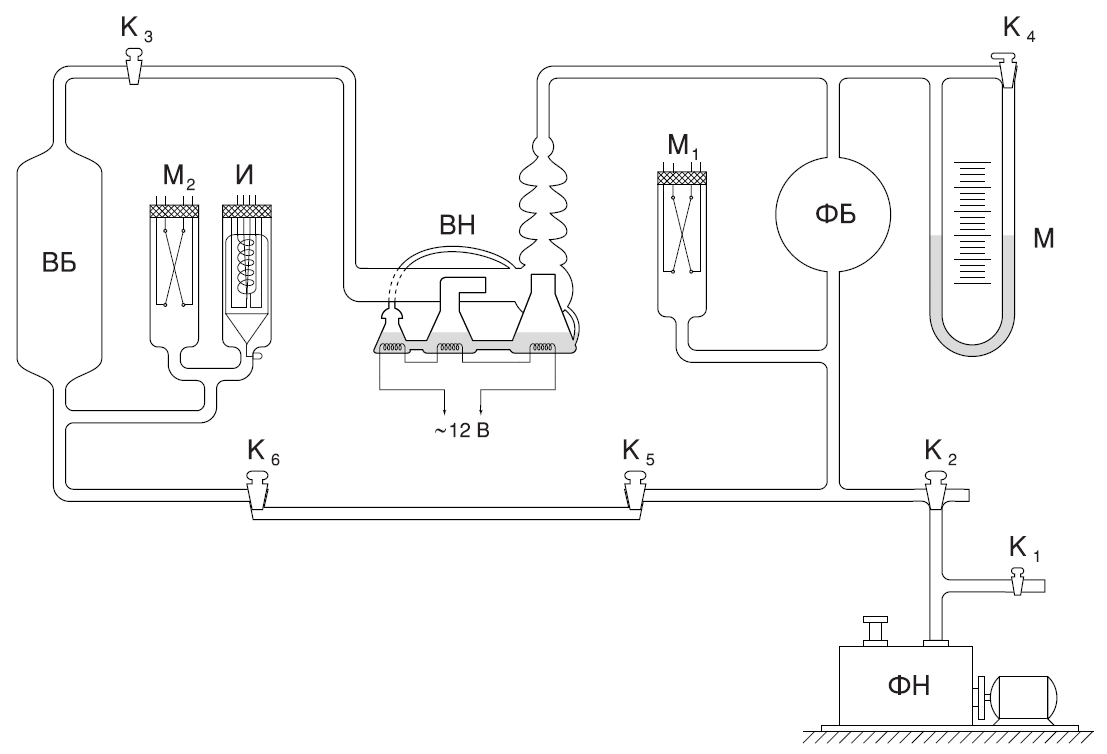
\includegraphics[width=0.7\linewidth]{установка.png}
 	\caption[]{Схема установки}
 
 \end{figure}
 
 
\noindent Все краны вакуумной установки стеклянные. Стенки кранов тонкие, пробки кранов полые и составляют одно целое с рукоятками. Пробки кранов притерты к корпусам. Для герметизации используется вакуумная смазка.

\medskip

\noindent Устройство и принцип действия \textbf{форвакуумного насоса} схематически, но довольно ясно изображены на рис 2. В положениях <<а>> и <<б>> пластина <<А>> засасывает разреженный воздух из откачиваемого объёма, а пластина <<Б>> вытесняет ранее захваченный воздух в атмосферу. В положениях <<в>> и <<г>> пластины поменялись ролями.

\begin{figure}[!h]
	\centering
	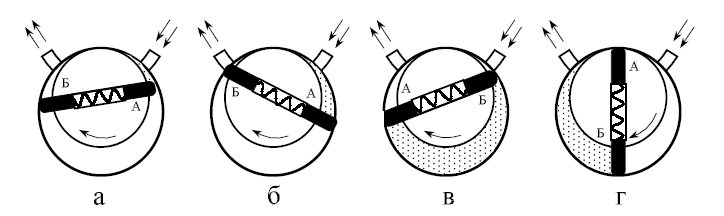
\includegraphics[width=0.9\linewidth]{фв.png}
	\caption[]{Схема действия ротационного двухпластинчатого форвакуумного насоса}
	
\end{figure}


\noindent Устройство и принцип действия \textbf{диффузионного насоса} схематически изображены на рис 2. Такой насос работает в тысячи раз быстрее форвакуумного. Его действие основано на диффузии. Масло, налитое в сосуд А, подогревается электрической печкой. Пары масла поднимаются по трубке Б и вырываются из сопла В. Струя паров увлекает молекулы газа, которые поступают из откачиваемого сосуда через трубку ВВ. В трубке Г мало осаждается и стекает вниз. Оставшийся газ, выходя в трубку ФВ, откачивается форвакуумным насосом.

\medskip

\noindent Диффузионный насос работает наиболее эффективно, когда длина свободного пробега молекул примерно равна ширине кольцевого зазора между соплом В и стенками трубки ВВ. Давление насыщенных паров масла при рабочей температуре, создаваемой обогревателем сосуда А, много больше $5\cdot 10^{-2}$ торр, поэтому пары масла создают плотную струю, увлекающую с собой молекулы газа.


\begin{figure}[!h]
	\centering
	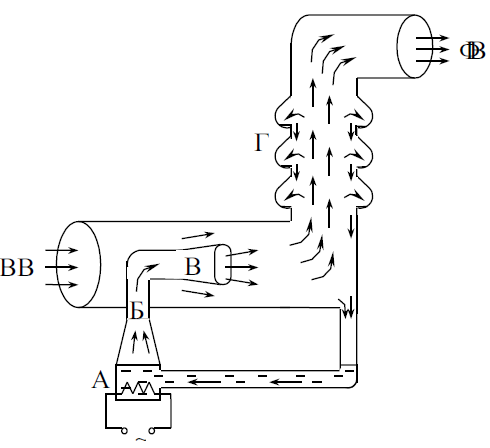
\includegraphics[width=0.4\linewidth]{вв.png}
	\caption[]{Схема работы диффузионного насоса}
	
\end{figure}


\noindent Диффузионный насос, используемый в нашей установке (см. рис 1) имеет две ступени и соответственно два сопла. Одно сопло вертикальное (первая ступень), второе горизонтальное (вторая ступень). За второй ступенью имеется ещё одна печь, но пар из этой печи поступает не в сопло, а по тонкой трубке подводится ближе к печке первой ступени. Эта печь осуществляет фракционирование масла. Легколетучие фракции масла, испаряясь, поступают в первую ступень, обогащая её. По этой причине плотность струи первой ступени выше, и эта ступень начинает откачивать при более высоком давлении в форвакуумной части. Вторая ступень обогащается малолетучими фракциями масла. Плотность струи второй ступени меньше, но меньше и давление насыщенных паров. Соответственно, в откачиваемый объем поступает меньше паров масла, и его удаётся откачать до более высокого вакуума.
 
 \begin{figure}[!h]
 	\centering
 	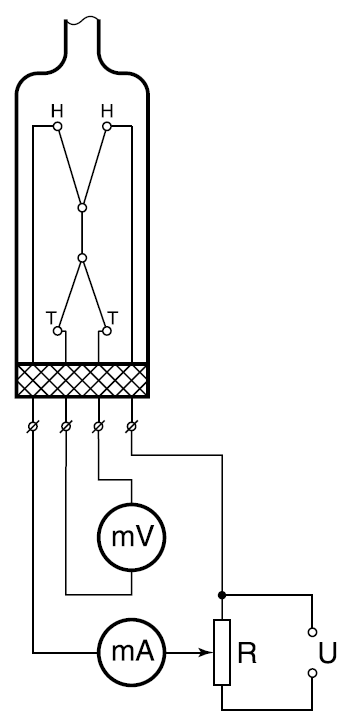
\includegraphics[width=0.2\linewidth]{термопара.png}
 	\caption[]{Схема термопарного манометра с лампой ЛТ-2}
 	
 \end{figure}
 
\medskip
 
\noindent \textbf{Термопарный манометр.} Чувствительным элементом манометра является платиново-родиевая термопара, спаянная с никелевой нитью накала и заключённая в стеклянный баллон. Устройство термопары пояснено на рис. 4. По нити накала НН пропускается ток постоянной величины. Для установки тока служит потенциометр R, расположенный на передней панели вакуумметра. Термопара ТТ присоединяется к милливольтметру, показания которого определяются температурой нити накала и зависят от отдачи тепла в окружающее пространство.

\medskip

\noindent Потери тепла определяются теплопроводностью нити и термопары, теплопроводностью газа, переносом тепла конвективными потоками газа внутри лампы, и теплоизлучением нити (инфракрасное тепловое излучение). В обычном режиме лампы основную роль играет теплопроводность газа. При давлениях, не меньших 1 торр, теплопроводность газа, а вместе с ней и ЭДС термопары практически не зависят от давления газа, и прибор не работает.

\medskip

\noindent При улучшении вакуума средний свободный пробег молекул становится сравнимым с диаметром нити, теплоотвод падает, и температура спая возрастает. При вакууме порядка $10^{-3}$ торр теплоотвод, осуществляемый газом, становится сравнимым с другими потерями тепла, и температура становится практически постоянной. Градуировочная кривая термопары приведена на рис. 5.


 \begin{figure}[!h]
 	\centering
 	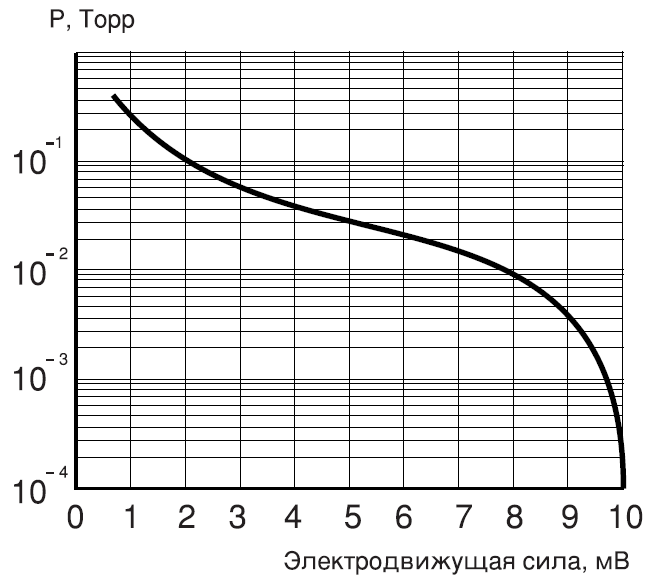
\includegraphics[width=0.4\linewidth]{градуировочная кривая.png}
 	\caption[]{Градуировочная кривая термопары ЛТ-2}
 	
 \end{figure}

		
\noindent \textbf{Ионизационный манометр.} Схема ионизационного манометра изображения на рисунке 6. Он представляет собой трехэлектродную лампу. Электроны испускаются раскалённым катодом и увлекаются электрическим полем к аноду, имеющему вид редкой спирали. Проскакивая за её витки, электроны замедляются полем коллектора и возвращаются к аноду. Прежде чем осесть на аноде, они успевают много раз пересечь пространство между катодом и коллектором. На своём пути электроны ионизуют молекулы газа. Ионы, образовавшиеся между анодом и коллектором, притягиваются полем коллектора и определяют его ток.

\begin{figure}[!h]
 	\centering
 	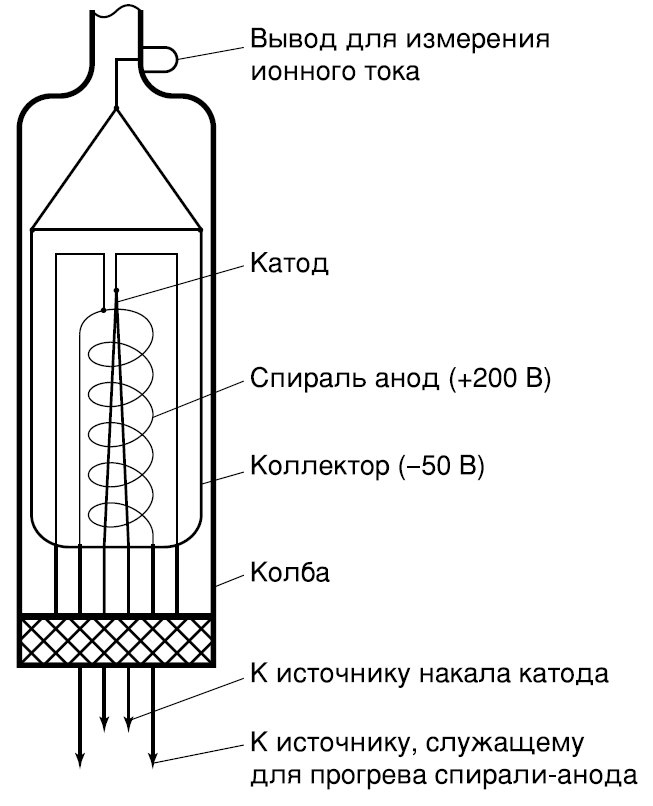
\includegraphics[width=0.3\linewidth]{лампа.png}
 	\caption[]{Схема ионизационной лампы ЛТ-2}
 	
 \end{figure}

\medskip

\noindent Накалённый катод ионизационного манометра перегорает, если давление в системе превышает $10^{-3}$ торр, поэтому перед его включением необходимо проверить давление термопарным манометром.
\medskip

\section{Теоретические сведения}

 \subsection*{Процесс откачки}
\noindent Опишем процесс откачки математически: 
Пусть W --- объем газа, удаляемого из сосуда при данном давлении за единицу времени, $Q_i$ для различных значений i обозначим различные притоки газа в сосуд (в единицах PV), такие как течи извне $Q_\text{и}$, десорбция с поверхностей внутри сосуда $Q_\text{д}$, обратный ток через насос $Q_\text{н}$. Тогда, приравнивая убыль газа из сосуда (с точностью до $RT/\mu$) в единицу времени $-VdP$ и сумму перечисленных токов имеем:

 \begin{equation}
 	-VdP = (PW - \sum_i Q_i)dt
 \end{equation}
 
\noindent При достижении предельного вакуума устанавливается давление $P_{\text{пр}}$, и $dP = 0$. Тогда
 
 \begin{equation}
 	 W = ( \sum_i Q_i )/P_{\text{пр}}
 \end{equation}
 
\noindent Поскольку обычно $Q_\text{и}$ постоянно, а $Q_\text{н}$ и $Q_\text{д}$ слабо зависят от времени, также считая постоянной W, можем проинтегрировать (1) и получить:
 
 \begin{equation}
 	P - P_{\text{пр}} = (P_0 - P_{\text{пр}})\exp(-\frac{W}{V}t)
 \end{equation}
 
\noindent Полная скорость откачки $W$, собственная скорость откачки насоса $W_{\text{н}}$ и проводимости элементов системы $C_1, C_2,...$ соотносятся согласно формуле (4), и это учтено в конструкции установки.

 \begin{equation}
 \frac{1}{W} = \frac{1}{W} + \frac{1}{C_1} + \frac{1}{C_2} + ...
\end{equation}

\subsection*{Течение газа через трубу}

\noindent Характер течения газа существенно зависит от соотношения между размерами системы и длиной свободного пробега молекул. При атмосферном и форвакуумном давлениях  длина свободного пробега меньше диаметра трубок, и течение газа определяется его вязкостью, т.е. взаимодействием молекул. При высоком вакууме течение существеннее определяется взаимодействием со стенками.

\medskip

\noindent Для количества газа, протекающего через трубу длины $l$ и радиуса $r$ в условиях высокого вакуума, справедлива формула:

\begin{equation}
	\frac{d(PV)}{dt} = \frac{4}{3}r^3\sqrt{\frac{2\pi RT}{\mu}}\frac{P_2 - P_1}{l}
\end{equation}

\noindent Если труба соединяет насос установку, то давлением $P_1$ у насоса можно пренебречь. Давление в сосуде $P = P_2$. Тогда имеем:

\begin{equation}
C_\text{тр} = \left(\frac{dV}{dt}\right)_\text{тр} = \frac{4r^3}{3l}\sqrt{\frac{2\pi RT}{\mu}}
\end{equation}

\noindent Для пропускной способности отверстий имеется формула

\begin{equation}
C_\text{отв} = \left(\frac{dV}{dt}\right)_\text{отв} = S\frac{\bar{\upsilon}}{4}
\end{equation}

\noindent Для воздуха при комнатной температуре $\bar{\upsilon}/4 = 110~\text{м/с} = 11~\text{л/c}\cdot\text{см}^2$.

\medskip

\section{Ход работы}

\subsection*{Измерение объёмов форвакуумной и высоковакуумной частей установки}

\noindent 1. Проверим, что $K_4$ открыт, впустим в установку атмосферный воздух через краны $K_1$ и $K_2$. <<Запрем>> в капилляре атмосферный воздух кранами $K_5$ и $K_6$. Объем капилляра в используемой установке: $$V_\text{к} = 50~ \text{см}^3.$$

\noindent 2. Закроем $K_1$ и $K_2$, включим форвакуумный насос и дадим ему откачать себя. Подключим установку к насосу краном $K_2$. Откачаем установку до $P = 1,7 \cdot 10^{-2}$ торр. Отсоединим установку краном $K_2$, и оставим насос работать <<на себя>>. Перекроем  $K_3$, отделяя высоковакуумною часть установки. Закроем $K_4$ для подготовки масляного манометра к измерениям.

\medskip

\noindent 3. Откроем  $K_5$, чтобы <<запертый>> ранее воздух заполнил форвакуумную часть установки, снимем давление с помощью вакуумного манометра, измерив разность высот столбиков масла:

$$ h_1 = (12.8\pm0.1) ~\text{см};\quad h_2 = (39.2\pm0.1) ~\text{см}$$
		
$$\Delta h_\text{фв} = (26.9\pm0.1) ~\text{см}$$	

\medskip

\noindent 4. Имея в виду, что плотность масла в манометре равна $ \rho = 885 \text{ г/л}$, а $P_\text{атм} = 101.3 \text{ кПа}$, и пользуясь законом Бойля-Мариотта, получим:

$$ V_\text{фв} = V_\text{к} \frac{P_\text{атм}}{\Delta h_\text{фв} \rho g} = (2.13\pm0,01)~\text{л} $$

\noindent 5. Аналогично, открыв кран $K_3$, получим значения разности высот на манометре

$$h_3 = (18.0\pm0.1) \text{ см};\quad h_4 = (39.7\pm0.1) \text{ см},$$

$$\Delta h_\text{полн} = (17.2\pm0.1) ~\text{см}$$
		
\noindent Получим полный объем и объем высоковакуумной части установки:

$$ V_\text{полн} = V_\text{к} \frac{P_\text{атм}}{\Delta h_\text{полн} \rho g} = (3.33\pm0,01)~\text{л}$$

$$ V_\text{вв} = V_\text{полн} - V_\text{фв} = (1,20\pm0,02)~\text{л} $$

\noindent 6. Откроем кран $K_4$, чтобы уравновесить масло в манометре во избежание его переброса в установку.
		
\medskip

\subsection*{Получение высокого вакуума}

\noindent 1. Продолжим откачивать установку форвакуумным насосом. Включим термопарный вакуумметр ВИТ-2 и по градуировочной кривой проверим ЭДС. После того, как давление упадёт примерно до $2\cdot10^{-2}$ торр, закроем краны К5 и К6 и приступим к откачке высоковакуумной части насоса с помощью диффузионного насоса. По вакуумметру ВИТ-2 пронаблюдаем за процессом откачки высоковакуумного баллона, необходимо достигнуть давления порядка 10$^{-4}$ торр, что соответствует ЭДС 10 mV. Когда стрелка прибора достигнет этого значения, закроем кран К6.

\medskip

\noindent 2. При выключенной ионизационной лампе, вставив предохранитель, ставим переключатель <<Род работы>> в положение <<Обезгаживание>> на 10 минут.

\medskip

\noindent 3. Включим ионизационную лампу.

\medskip

\noindent 4. Измерим предельное давление:

	$$P_{\text{пр}} = 6,2\cdot10^{-5} ~\text{торр}$$	

\subsection*{Измерение скорости по ухудшению и улучшению вакуума}

\noindent 1. Закроем К3 и запишем на видео ухудшение и улучшение вакуумаспо времени по изменению показаний ионизационного манометра (Таблица 1). Полученные результаты изобразим на графиках (Рис. 7 и 8).

\medskip

\noindent Рассчитав коэффициенты наклона графиков и зная объем высоковакуумной части установки, получим скорость откачки W диффузионного насоса. Считаем $$W = -\bar{k}\cdot V_\text{вв}, \quad\varepsilon_W^2 = \varepsilon_{\bar{k}}^2 + \varepsilon_{V_\text{вв}}^2,$$  где $\bar{k}$ --- среднее коэффициентов наклона).

\medskip

\noindent По ухудшению:
	$$W = (0,44\pm0,03) ~\text{л/с}$$
	
\medskip	
	
\noindent По улучшению:
	$$W = (0,25\pm0,02) ~\text{л/с}$$

\medskip

\noindent 2. Оценим пропускную способность трубки от высоковакуумного баллона до насоса.

\medskip

\noindent Для случая ухудшения вакуума оценим $Q_\text{н}$ c помощью полученных зависимостей P(t). Считаем $$\frac{dP}{dt} = \bar{k}$$ где $\bar{k}$ --- среднее коэффициентов наклона из зависимостей P(t). Имеем:
	$$Q_\text{н} + Q_\text{д} = (1,26\pm0,04)\cdot 10^{-5} ~\text{торр}\cdot\text{л/c}$$
	\noindent Таким образом,
	$$Q_\text{н} + Q_\text{д} \approx 1,26\cdot 10^{-5} ~\text{торр}\cdot\text{л/c}$$

\noindent Оценим пропускную способность
  $$d \sim 10^{-2}~\text{м},\quad L \sim 1 ~\text{м},\quad \sqrt{\frac{RT}{\mu}} \sim 500 ~\text{м/с},$$ 
	 Имеем:
	$$C_\text{тр} \sim 1 ~\text{л/с},$$

\medskip

\noindent 3. Рассчитаем производительность насоса ещё одним способом: создав искусственную течь. Откроем кран $K_6$ при включённом  насосе и измерим давление, установившееся при течи.
 $$P_\text{уст} = 1,5 \cdot 10^{-4} ~\text{торр}.$$

		$$P_\text{пр}W = Q_1, \quad P_\text{уст}W = Q_1 + \frac{(PV)_\text{капилляр}}{dt}$$
		
$$(P_\text{уст} - P_\text{пр})W = \frac{4}{3}(d/2)^3\sqrt{\frac{2\pi RT}{\mu}}\frac{P_\text{фв}}{L},$$

\noindent где d и L --- диаметр и длина капилляра
	$$d = 0,8 ~\text{мм},\quad L = 10,8 ~\text{см}$$
	
	$$P_\text{фв}= 3,4 \cdot 10^{-3} \text{ торр}$$

\noindent Таким образом,
	$$W \approx 0,56 ~\text{л/c}.$$

\medskip

\section{Вывод}

В ходе работы:

\medskip
  
\noindent 1. Были определены объёмы форвакуумной и высоковакуумной частей установки. 

\medskip
 
\noindent Объём форвакуумной части $V_\text{фв} = (2.13\pm0,01)~\text{л}$\\
\noindent Объём высоковакуумной части $V_\text{вв} = (1,20\pm0,02)~\text{л}$\\
\noindent Объём всей установки $V_\text{полн} = (3.33\pm0,01)~\text{л}$\\

\medskip

\noindent 2. Был получен высокий вакуум: $P = 6,2 \cdot 10^{-5}$ торр.

\medskip

\noindent 3. Определена скорость откачки по ухудшению и улучшению вакуума.

\medskip	

\noindent По ухудшению:
	$$W = (0,44\pm0,03) ~\text{л/с}$$
	
\medskip	
	
\noindent По улучшению:
	$$W = (0,25\pm0,02) ~\text{л/с}$$

\medskip

\noindent 4. Определена скорость откачки с помощью искусственно созданной течи.  $$W \approx 0,56 ~\text{л/c}.$$

\medskip

\subsection*{Таблицы и графики}
\medskip

\begin{center}
Таблица 1
\end{center}

\begin{center}
\begin{tabular}{|c|c|c|c|c|c|c|c|c|c|}
\hline 
\multicolumn{6}{|c|}{$\text{Ухудшение}$} & \multicolumn{4}{c|}{$\text{Улучшение}$} \\ 
\hline 
t, c & P, $\cdot 10^{-4} \text{торр}$ & t, c & P, $\cdot 10^{-4} \text{торр}$ & t, c & P, $\cdot 10^{-4} \text{торр}$ & t, c & P, $\cdot 10^{-4} \text{торр}$ & t, c & P, $\cdot 10^{-4} \text{торр}$ \\ 
\hline
27 & 1,6	 & 39 & 1,3 & 33 & 2,0 & 22 & 0,78 & 21 & 0,8\\
\hline
29 & 1,7	 & 44 & 1,8 & 41 & 2,8 & 27 & 0,74 & 24 & 0,77\\
\hline
30 & 1,8	 & 48 & 2,3 & 48 & 3,5 & 32 & 0,73 & 26 & 0,76\\
\hline
31 & 1,9	 & 53 & 2,7 & 54 & 4,2 & 35 & 0,73 & 30 & 0,75\\
\hline
34 & 2,2	 & 58 & 3,2 & 61 & 4,8 & 37 & 0,72 & 33 & 0,74\\
\hline
36 & 2,3	 & 64 & 3,7 & 68 & 5,5 & 45 & 0,71 & 36 & 0,73\\
\hline
39 & 2,6	 & 69 & 4,3 & 76 & 6,2 & 51 & 0,70 & 39 & 0,72\\
\hhline{----------}
42 & 2,9	 & 75 & 4,8 & \multicolumn{2}{|c|}{ } & 54 & 0,70 & 42 & 0,72\\
\hhline{----~~----}
44 & 3,0	 & 82 & 5,5 &  \multicolumn{2}{|c|}{ }  & 58 & 0,69 & 46 & 0,73\\
\hhline{----~~----}
49 & 3,5	 & 87 & 6,0 &  \multicolumn{2}{|c|}{ }  & 61 & 0,695 &  \multicolumn{2}{|c}{ } \\
\hhline{----~~--~~}
54 & 3,9	 &  \multicolumn{8}{|c}{ } \\
\hhline{--~~~~~~~~}
59 & 4,4	 &  \multicolumn{8}{|c}{ } \\
\hhline{--~~~~~~~~}
64 & 4,8	 &  \multicolumn{8}{|c}{ } \\
\hhline{--~~~~~~~~}
69 & 5,2	 &  \multicolumn{8}{|c}{ } \\
\hhline{--~~~~~~~~}
74 & 5,7	 &  \multicolumn{8}{|c}{ } \\
\hhline{--~~~~~~~~}
80 & 6,2	 &  \multicolumn{8}{|c}{ } \\
\hhline{--~~~~~~~~}
93 & 7,4	 &  \multicolumn{8}{|c}{ } \\
\hhline{--~~~~~~~~} 
\end{tabular} 
\end{center}

\medskip

\begin{figure}[h]
\center{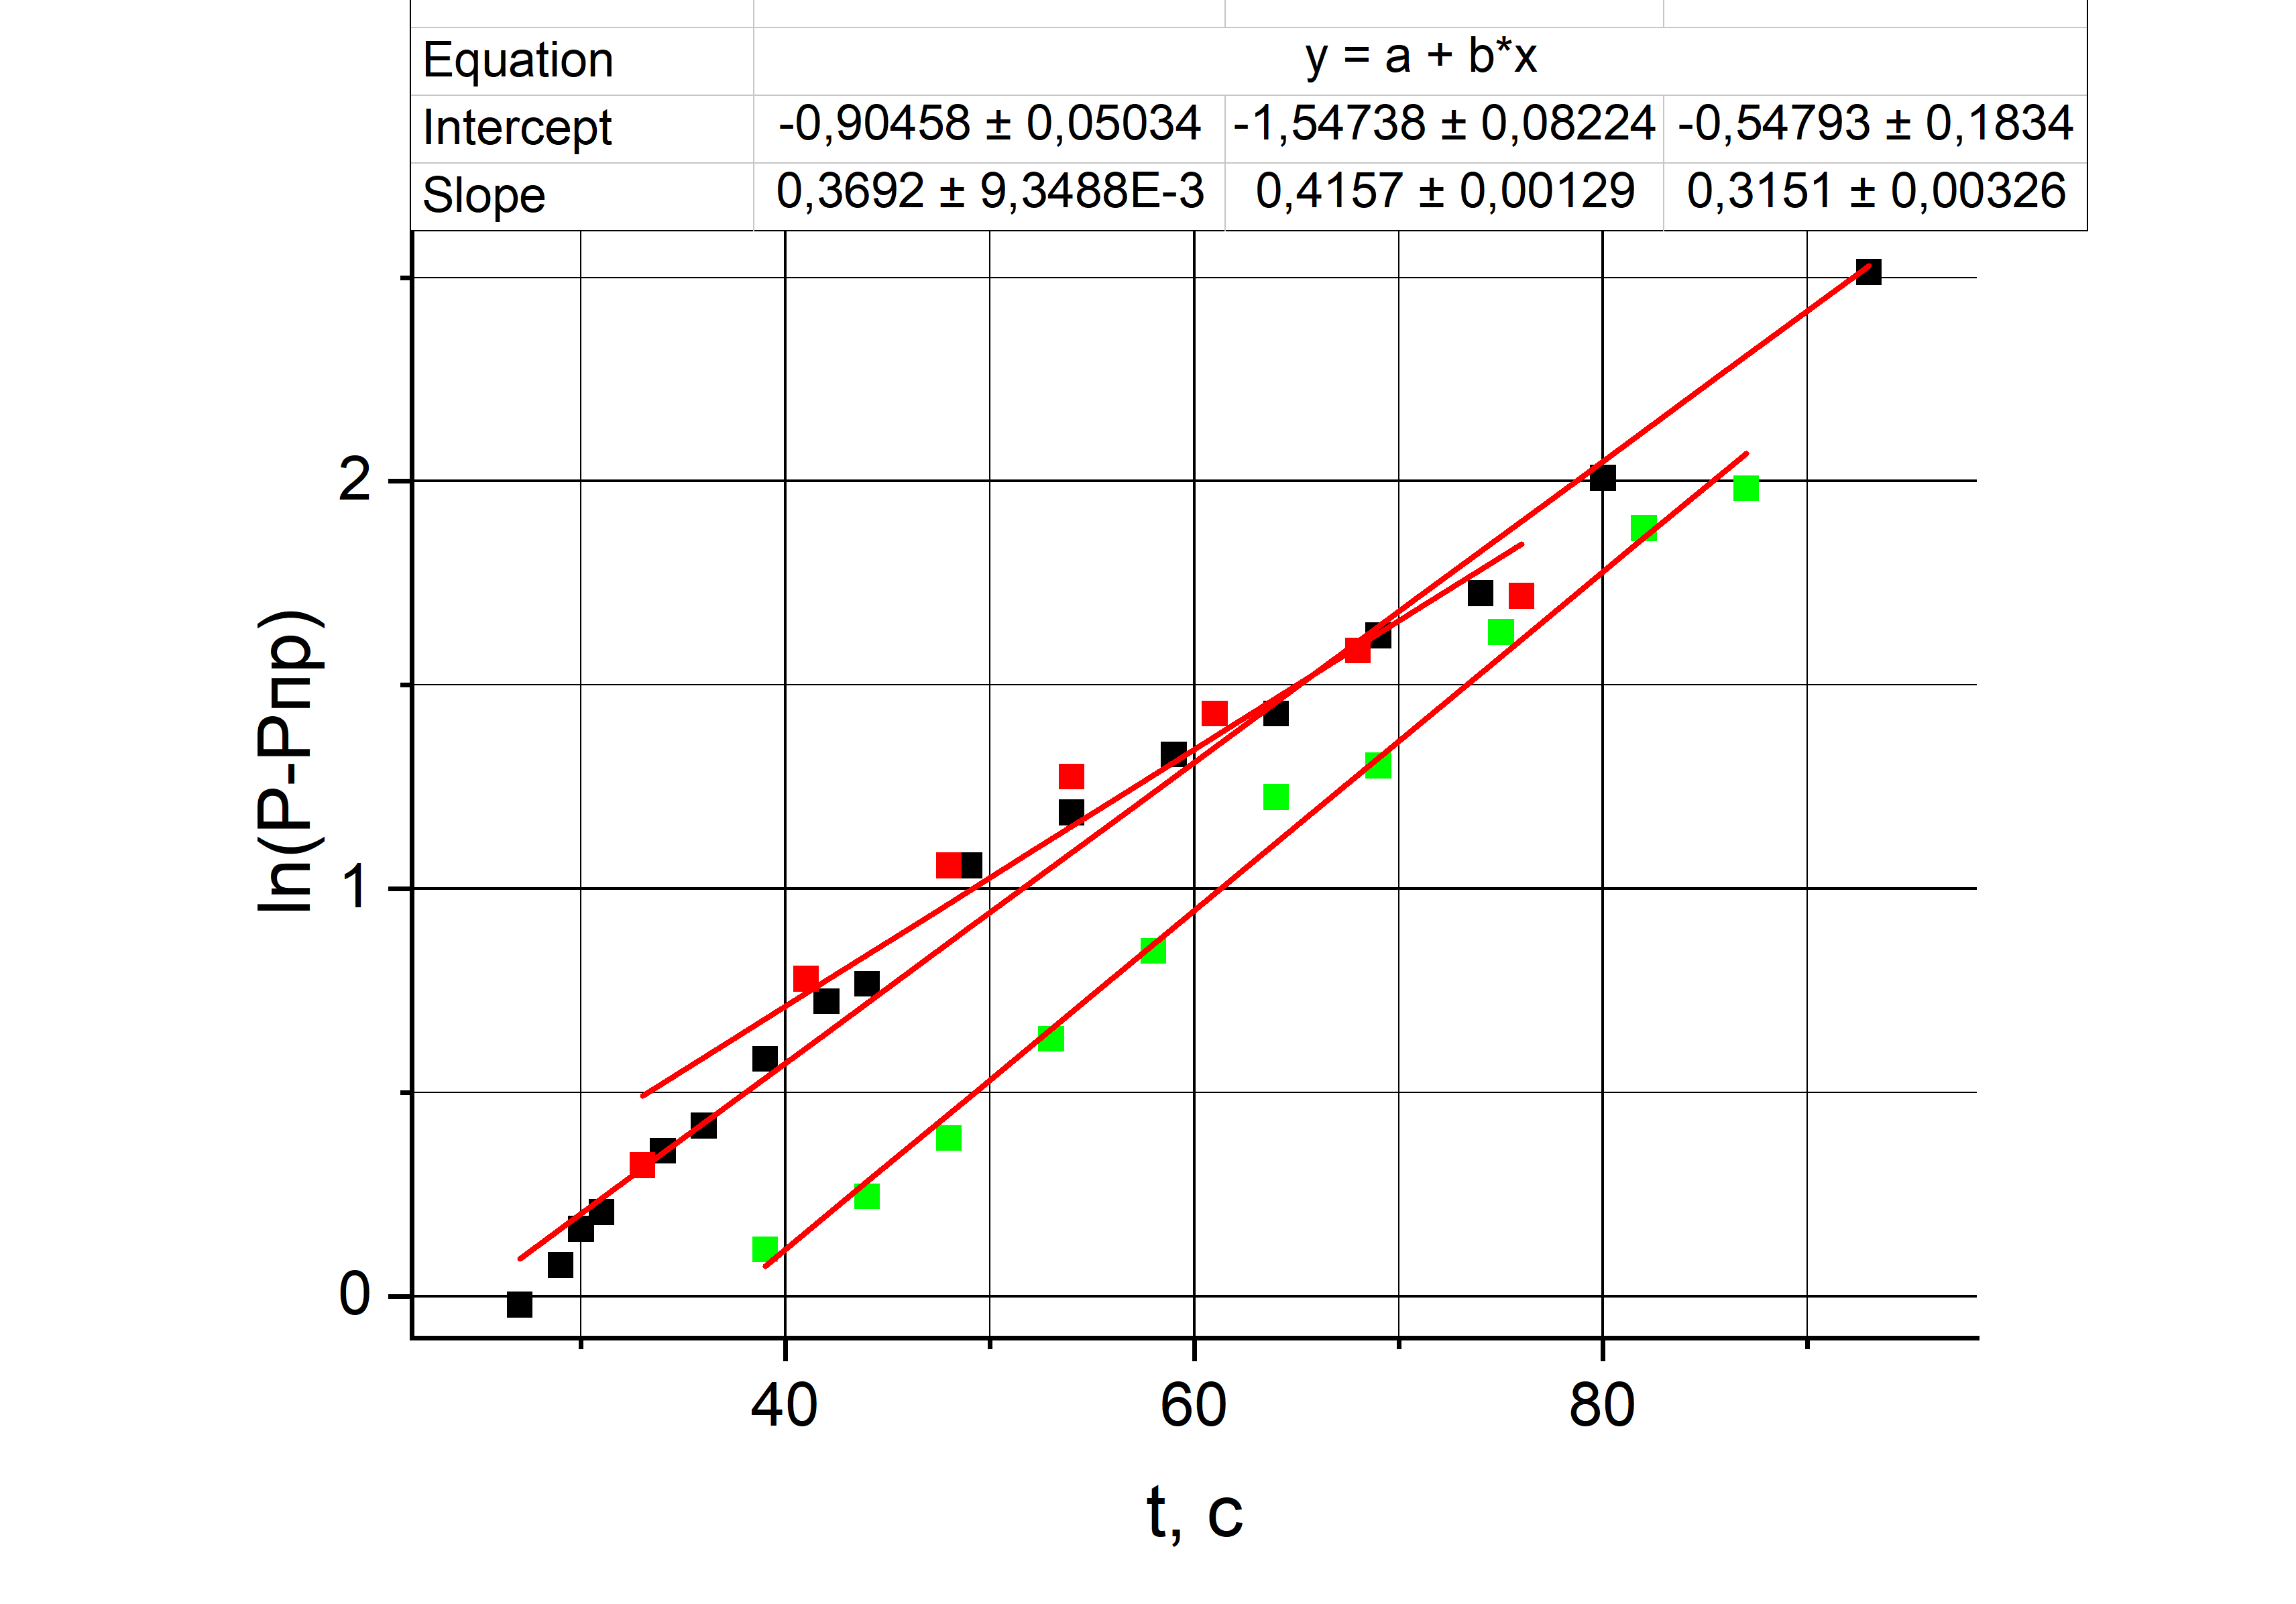
\includegraphics[scale={0.5}]{ухудшение.png}}
\caption{Зависимость давления от времени при ухудшении вакуума}
\end{figure}

\begin{figure}[h]
\center{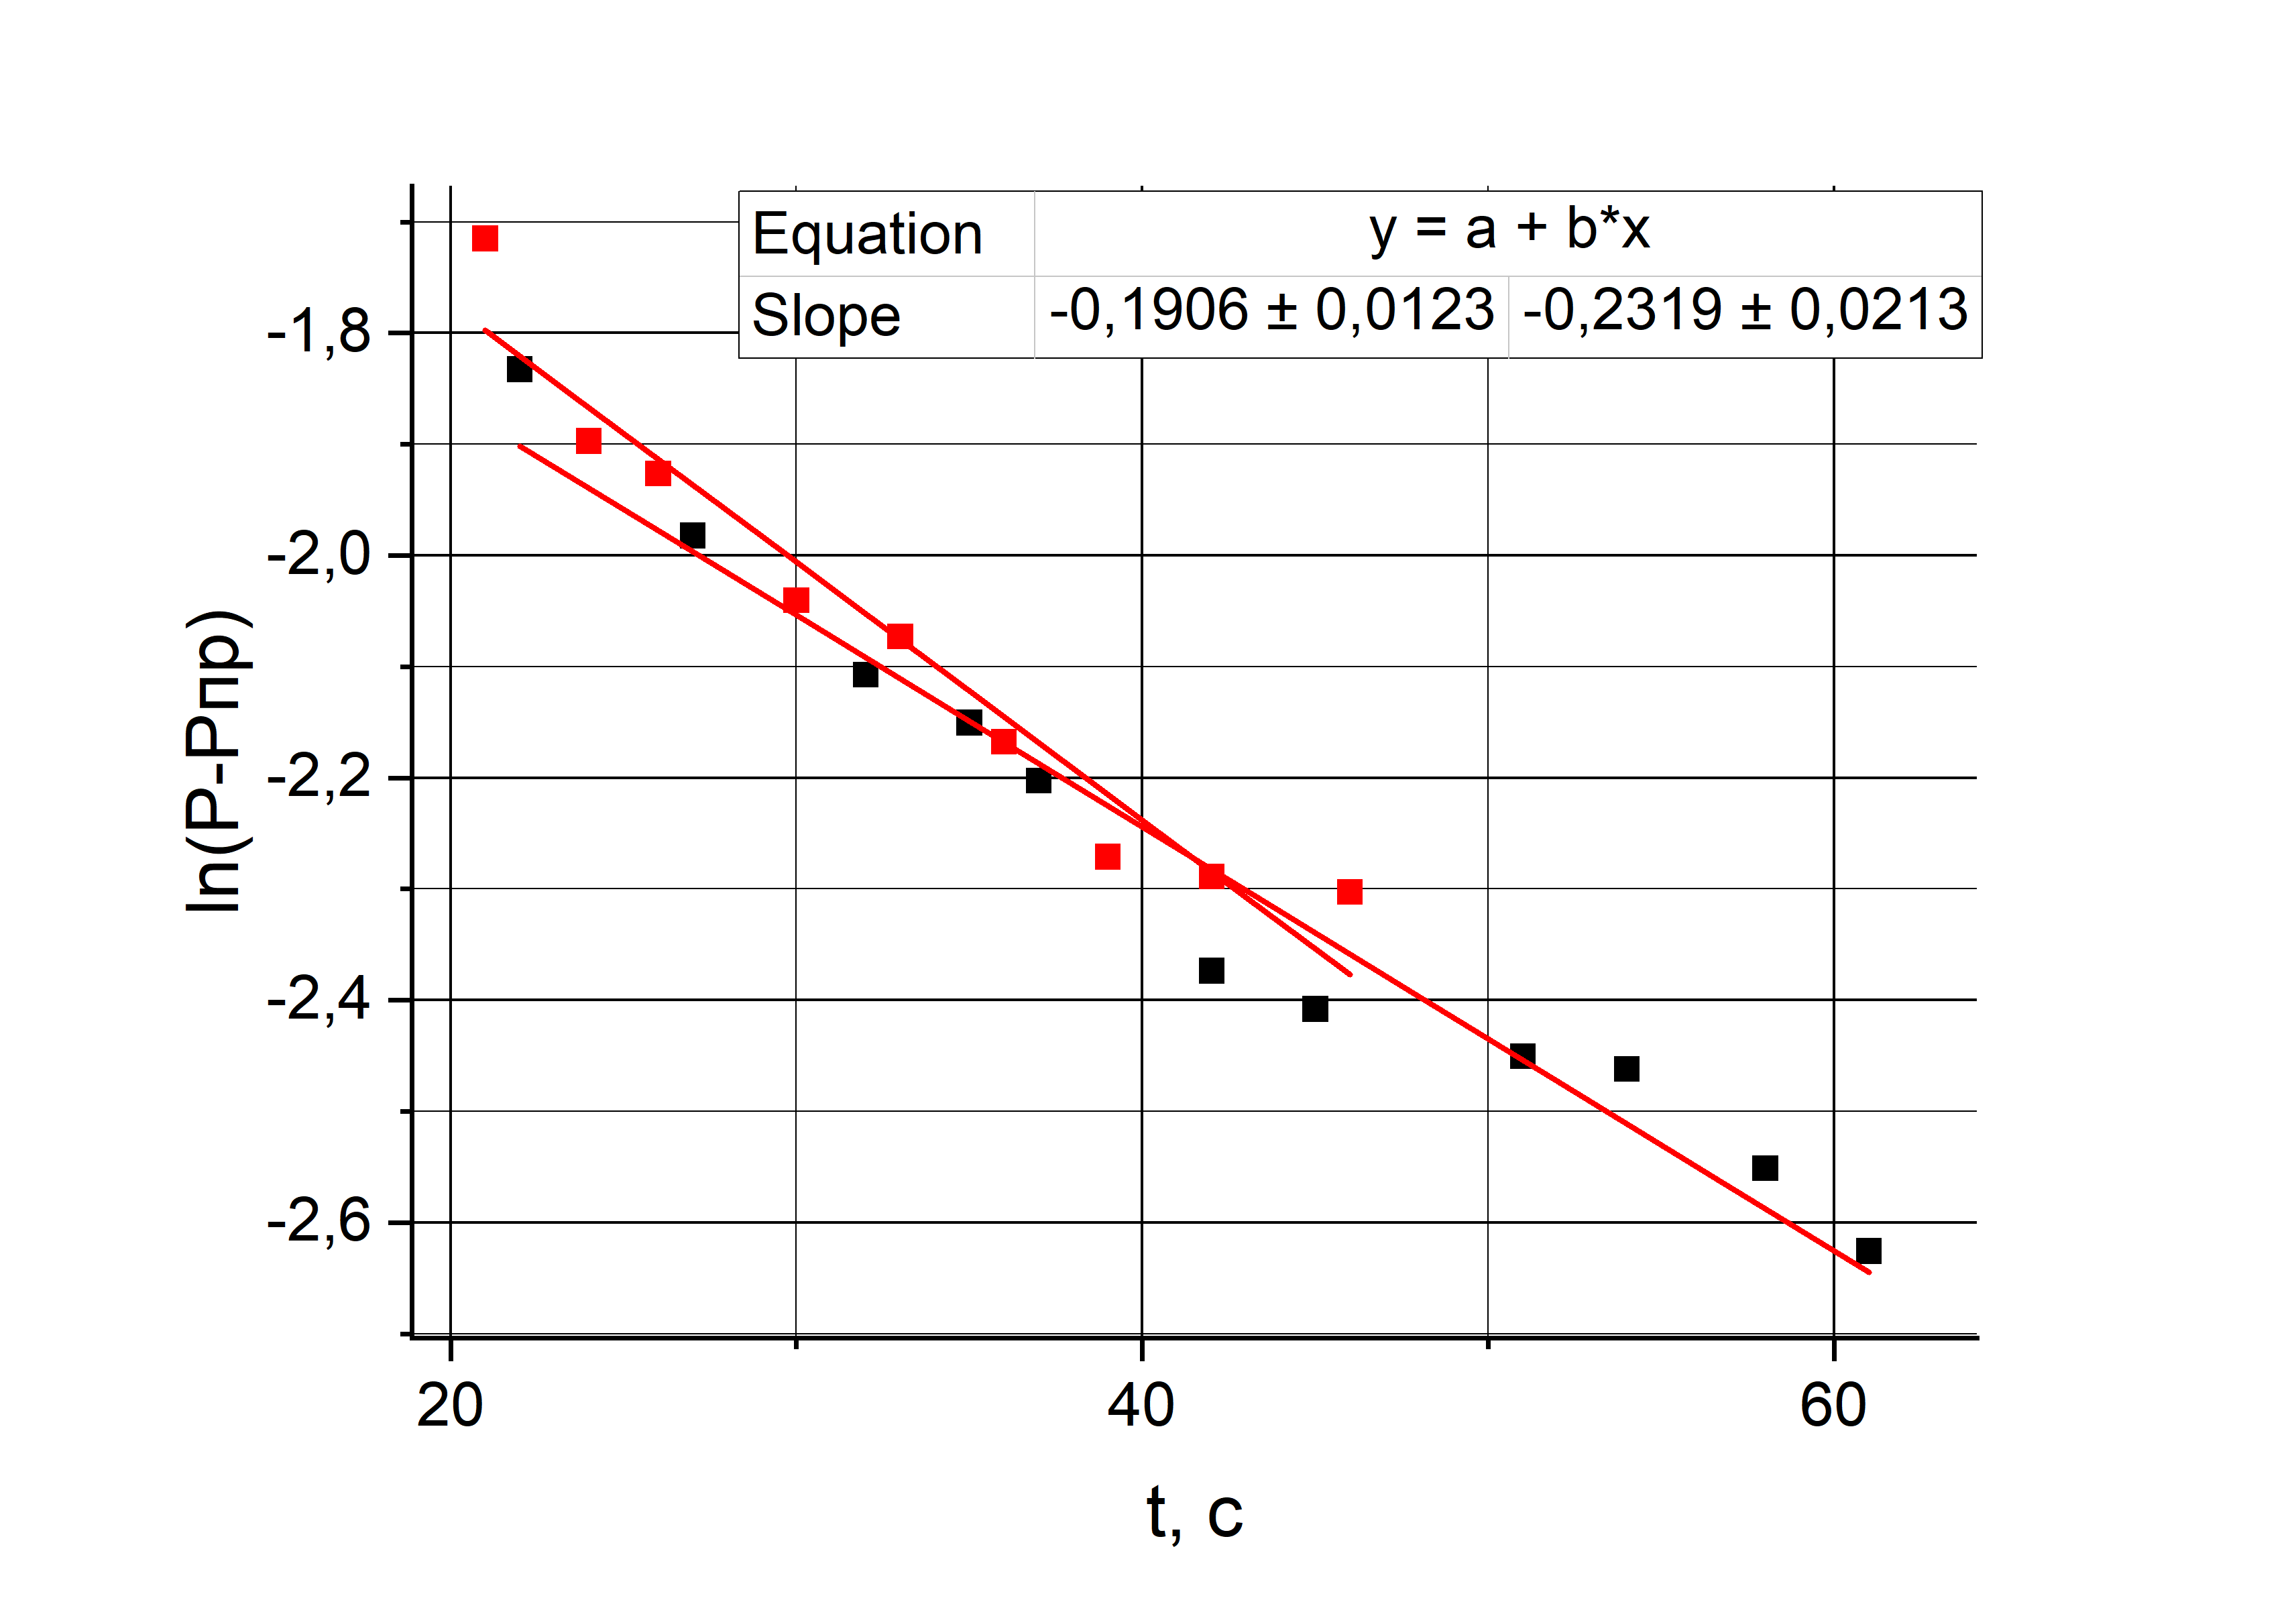
\includegraphics[scale={0.5}]{улучшение.png}}
\caption{Зависимость давления от времени при улучшении вакуума}
\end{figure}


\medskip

\end{document}